\chapter{Computational Frameworks}

\section{Background}
\quad For many decades there has been an ongoing trend in the process of software engineering to move up in the levels of abstraction from a bare hardware to a higher level concepts closer to a human reasoning and understanding. There have been several breaking points. A move from assembly languages to languages like Fortran and C increased the productivity of programmers by supporting structuredness and modularity and offloading many routine and tedious tasks onto a compilation software. C and Fortran were high-level languages of that time, but still a low-level languages for today's standards. These languages support an imperative programming paradigm. The main characteristic of that is the concept of state. The statements of the language read and update the state. Procedures pass the state and results around achieving the final goal of the program.   

\quad The trend of moving from low to higher abstraction levels is not only true for software engineering in general, but for parallel software engineering in particular. Modern hardware provides a diverse and vast support for different forms of parallelism: pipelined CPUs with out-of-order and superscalar instruction execution, vector extensions of modern CPU instruction sets, multi-core processors running as part of multi-processor system, etc. Given a sequential program a programmer can work at the finest level of granularity by choosing vector instructions over scalar ones and changing their relative order trying to minimise the number of pipeline stalls and memory waits. To exploit a coarse-grain parallelism a programmer can rewrite a program in a multi-threaded fashion. Here a programmer may choose to work with the operating system interface like POSIX threads or use some 

abstract parallel machine models   


level by rewriting program instructions by preferring vector ones to a scalar or change their relative order trying to minimise the number of pipeline stalls    

in modern computing systems a programmer may 

sequential program a programmer can work with its instructions directly by 



\subsection{Data-Centric Parallelization}
\label{chapter_dcp}
\subsubsection{The Problem}
\quad As it has already been stated the problem of software parallelisation is multifaceted. There is a vast range of lower level technical issues, which can turn a perfectly parallelisable at a higher level computation into a non-parallelisable implementation. In our ML assistant project (see Chapter \ref{chapter_ml_assistant}) we showed that the main reasons of Intel Compiler failures on SNU NPB benchmarks are alias analysis conservativeness, uninlined function calls and statically unresolvable dependencies. The assistant tool we designed targets these aspects of the software parallelisation problem. But, there are many more reasons leading to non-parallelisable algorithm implementations. Source code listings \ref{lst:array} and \ref{lst:list} brightly illustrate yet another unsolved problem.\newline\null
\begin{minipage}[t]{0.45\linewidth}
\begin{lstlisting}[caption={Parallelisable loop operating on a \textbf{linear array}.},label={lst:array},language=C]
for (int i=0; i<n; it++) {
  a[i]=a[i]+1;
}
\end{lstlisting}
\end{minipage}
%
\begin{minipage}[t]{0.55\linewidth}
\begin{lstlisting}[caption={Non-parallelisable loop operating on a \textbf{linked-list}.},label={lst:list},language=C]
for (p=list; p!=NULL; p=p->next) {
  p->value+=1;
}
\end{lstlisting}
\end{minipage}
\quad Listings \ref{lst:array} and \ref{lst:list} illustrate two alternative implementations of the same simple computation. We increment all sequence elements by one. Listing \ref{lst:array} implements the sequence with a regular array linearly laid out in the memory. Listing \ref{lst:list} chooses a linked list as an implementing data structure, which leads to a source code non-parallelisability.\newline\null
\quad In the project of "Data-Centric Parallelisation (DCP)" we would like to automatically recognise 
\subsubsection{Literature Review}
\label{dcp_literature_review}
\quad The idea of automatic discovery of higher level entities in programs is not a new one. This discovery problem is closely interlinked and entangled with alias analysis techniques \cite{Muchnick:1998:ACD:286076} like points-to analysis \cite{Emami:1994:CIP:178243.178264}. Points-to analysis is a variation on data flow analysis techniques. The final output is the sets of pairs of the form (\textit{p},\textit{x}) (pointer variable \textit{p} points to a stack allocated variable \textit{x}). These techniques are aimed at getting aliasing information regarding stack-allocated pointers.\newline\null
\quad The problem of understanding heap-directed pointers and heap-allocated linked data structures these pointers might point to is addressed with a family of static analysis techniques collectively known as shape analysis. Shape analysis techniques can be used to verify properties of dynamically allocated data structures in compile time. These are among the oldest and most well known techniques. Three-valued logic \cite{Sagiv:1999:PSA:292540.292552}\cite{Wilhelm:2000:SA:647476.760384} can be used as an example. The technique proposes a construction of a mathematical model consisting of logical predicate expressions. The latter correspond to certain pointer operating imperative language program statements. Abstract interpretation of these statements leads to a construction of sets of shape graphs at various program points. Shape graphs approximate the possible states of heap-allocated linked data structures and answer the questions such as node reachability, data structure disjointness, cyclicity, etc. The major limitation of these simplified mathematical models is the lack of precision high level of abstraction leads to. The problem of precise shape analysis is provably undecidable.\newline\null
\quad The work of \cite{Ghiya:1996:TDC:237721.237724} proposes a simplified and hence more practical implementation of shape analysis. Authors propose to use direction \textit{D} and interference \textit{I} matrices instead of complex mathematical models in order to derive shape information on heap allocated data structures. The entry of direction matrix \textit{D[p,q]} says if there exists a path from a node referred to by \textit{p} to a node referred to by q. In other words, if we can enter a path withing the data structure through \textit{p} and exit through \textit{q}. The entry of interference matrix \textit{I[p,q]} says if the paths started from \textit{p} and \textit{q} are going to intersect at some point. Authors implement their technique withing McCAT compiler, which uses SIMPLE intermediate representation with a total of 8 statements (\textit{malloc()}, pointer assignments \textit{p=q}, structure updates \textit{p-$>$next=q}), which are capable of changing \textit{D} and \textit{I} matrices. Statements generate and kill entries in matrices. Moreover, they are capable of changing \textit{Shape} attribute of pointers. The technique has been assessed on various benchmarks (bintree, xref, chomp, assembler, loader, sparse, etc.) from the era before the standard benchmark suites became available. The technique mostly reported shapes as \textit{Trees} (be it a binary tree or a linked-list) or sometimes as \textit{DAGs} or \textit{Cycles} but with higher error rates in these last cases. The latter shows that the technique is imprecise and conservative.\newline\null
\quad One of the more recent techniques designed and developed by Philip Ginsbach and Michael F. P. O’Boyle is based on the pattern matching on LLVM IR level. The main idea is to specify computational idioms to be recognized in a domain specific constraint based programming language CAnDL \cite{Ginsbach:2018:CDS:3178372.3179515}. Constraints are specified over LLVM IR entities such as instructions, basic blocks, functions, etc. The CAnDL language allows for a rapid prototyping of new compiler optimisations based on pattern recognition and its substitution with an optimised versions of matched idioms. The language and its relatively fast backtracking constraint solver are capable of recognizing not only simple arithmetic idioms (thus performing different peephole optimizations), but more complex computations like general reductions and histograms \cite{Ginsbach:2017:DEG:3049832.3049862}, vector products in graphics shaders \cite{Ginsbach:2018:AML:3296957.3173182}, sparse and dense linear algebra computations and stencils \cite{Ginsbach:2018:AML:3296957.3173182}. Having recognized these computational idioms the work \cite{Ginsbach:2018:AML:3296957.3173182} replaces them with a code for various heterogeneous APIs (MKL, libSPMV, Halide, clBLAS, CLBlast, Lift) and compares the resulting performance demonstrating an improvement over sequential versions and matching performance to a hand-written parallel versions. The technique has been deployed on the sequential C versions of SNU NPB, the C versions of Parboil and the OpenMP C/C++ versions of Rodinia demonstrating an improved detection capabilities over the state-of-the-art techniques.\newline\null
\quad The other principally different technique has been recently proposed by Changhee Jung and Nathan Clark \cite{1669122}. The authors developed a Data-structure Detection Tool (DDT) based on LLVM framework. The tool instruments loads, stores and calls withing program binaries and gathers dynamic traces for sample inputs. The traces are used to recreate a memory allocation graph for program data structures. Call graphs are used to identify interface functions interacting with the built memory graph. DDT traces memory graph properties (number of nodes, edges, etc.) before and after interface function calls into another Daikon tool to compute dynamic invariants (the number of nodes in a memory graph decreses by 1 after every \textit(delete()) interface method call, etc.). At the end manually constructed decision tree is used to probabilistically match observed behavioral patterns against known data structure invariant properties. The technique has been deployed to recognise data structure implementations withing standard libraries like STL, Apache (STDCXX), Borland (STLport), GLib, Trimaran achieving almost perfect recognition accuracy. Moreover, the technique has been able to recognise linked lists in Em3d and Bh Olden benchmarks, along with red-black trees implementing vectors in Xalancbmk benchmark.\newline\null
\quad There has recently been other published works on the application of dynamic techniques to the problem of dynamic data structure recognition \cite{Rupprecht:2017:DID:3155562.3155607}\cite{Haller:2016:SDS:2938006.2938029}. The technique used in the DDT tool \cite{1669122} makes an assumption, that all modifications and interactions with memory graphs representing data structures happen through a set of interface functions. That is not true, when we deal with aggressively optimising compilers, which may eliminate some code or inline some functions. The MemPick tool \cite{Haller:2016:SDS:2938006.2938029} searches data structures directly on a built dynamic memory graph by analyzing its shape. The graph is built with the help of Intel Pin binary instrumentation tool during quiescent periods, when pointer operations are absent. DSIbin tool \cite{Rupprecht:2017:DID:3155562.3155607} operates with the source code rather than program binaries. Instead of memory points-to graphs it uses strands as primitives, which abstract such entities as singly-linked lists.\newline\null
\quad The work of Dekker \cite{Dekker:1994:ADS:3107859.3107876} addresses software design recovery problem in a completely different way. Contrary to the approaches described above, which operate on the IR and dynamic instruction stream levels, work of Dekker operates at the level of abstract syntax tree. Dekker's tool tries to compact the tree down to a recognizable syntactic patterns by transforming it in accordance to a special grammar.


\subsection{OOP and Software Design Patterns}
\quad Object-oriented software design is a complex topic in itself, which spawns a number of problems and questions. 

\quad Software design patterns are reusable solutions to common design problems in object-oriented software engineering. They live at the level higher than that of a source code and are language agnostic. The solutions can be regarded as standard solutions to design problems they target. These solutions have been well tested and proven to be the most reliable and elegant.

Chain of responsibility pattern is very similar to fold.
Visitor pattern roughly corresponds to fold.

\subsection{Imperative and Functional programming}
\quad Programming languages can be classified by different programming paradigms they support. Among the most general classifications are imperative and declarative programming paradigms.\newline\null
\quad Imperative programs are written in a form of instruction sequences, which read and write the state of a program. The concept of state is the main characteristic of imperative programming paradigm. Instruction sequences can be structured in various ways. In procedural programming paradigm instructions are grouped inside procedures and functions. In object-oriented programming (OOP) paradigm instructions are grouped with the data they operate on inside objects of various types or classes.\newline\null
\quad Declarative programs do not specify the exact sequence of steps and state updates a program needs to do in order to get the desired result. Declarative programs declare the properties of the desired result. The properties can be specified as a set of constraints like in constraint programming or a set of linear inequalities like in linear programming. Functional programming is another subtype of declarative programming. In functional programming the final desired result is specified as a sequence of stateless function evaluations. Among the most common functions are map, reduce, fold, etc.

\subsection{Parallel Algorithmic Skeletons}




\section{Computational Frameworks}
\quad In this work we propose an idea of \textbf{computational frameworks} and we show its utility and use on a subset of Olden benchmarks. The idea grows on a wide review of the available parallel software development methodologies as well as on the understanding of problems in the task of software parallelization.  

\subsection{Overview}
\quad In our project we propose a C++ library of computational frameworks. Computational frameworks are a blend of imperative, object-oriented and functional programming paradigms. They lift algorithm implementation in the C++ language to a higher level.
Computational frameworks are a blend of algorithms and data structures as well as several programming paradigms such as imperative, object-oriented and functional programming. They lift C++ program implementations to a higher conceptual level. 

User-exposed methods of classes are higher-order functions and can take custom function objects, function pointers, lambda functions and apply them to framework elements in a framework defined way. Unlike pure functions the application of user-defined functions to our computational frameworks can have side-effects.

\quad Improves structuredness, modularity, separation of concerns and hides possible program parallelization behind the convenient user API.  

\subsection{Fractal}
\quad The \textbf{Fractal} computational framework has been inspired by the theoretical work on tree reductions [] and 3 Olden benchmarks (health, treeadd, perimeter). Figure \ref{fig:fractal} illustrates the Fractal functionality.\newline\null
\quad There are numerous data structures, computational patterns, processes and examples, which can be characterized as being fractals.\newline\null
\quad The simplest example of fractal is an n-ary tree. Imagine we store some data at every node of the tree and want to accumulate it starting from the leaves at the very bottom and going all the way up to the root of the tree. Accumulation procedure processes every node by taking the result from all its children, making a computation and passing the result up to the parent element. The procedure may have some side-effects on the nodes and keeps the whole tree data structure along with its state in memory. In that sense it is not a stateless functional programming. At the same time the accumulation procedure can be passed as an argument to a higher-order compute function. The movement of data through the nodes of the tree from their children to their parents is the fixed and immutable part of an algorithm, whereas the accumulation procedure can be given as a parameter. The latter separates the algorithm into a well-structured user and library parts. The library part acts as a backbone and the user part grows on it. The computations described above lie at the basis of health and treeadd benchmarks.\newline\null
\begin{figure}[ht]
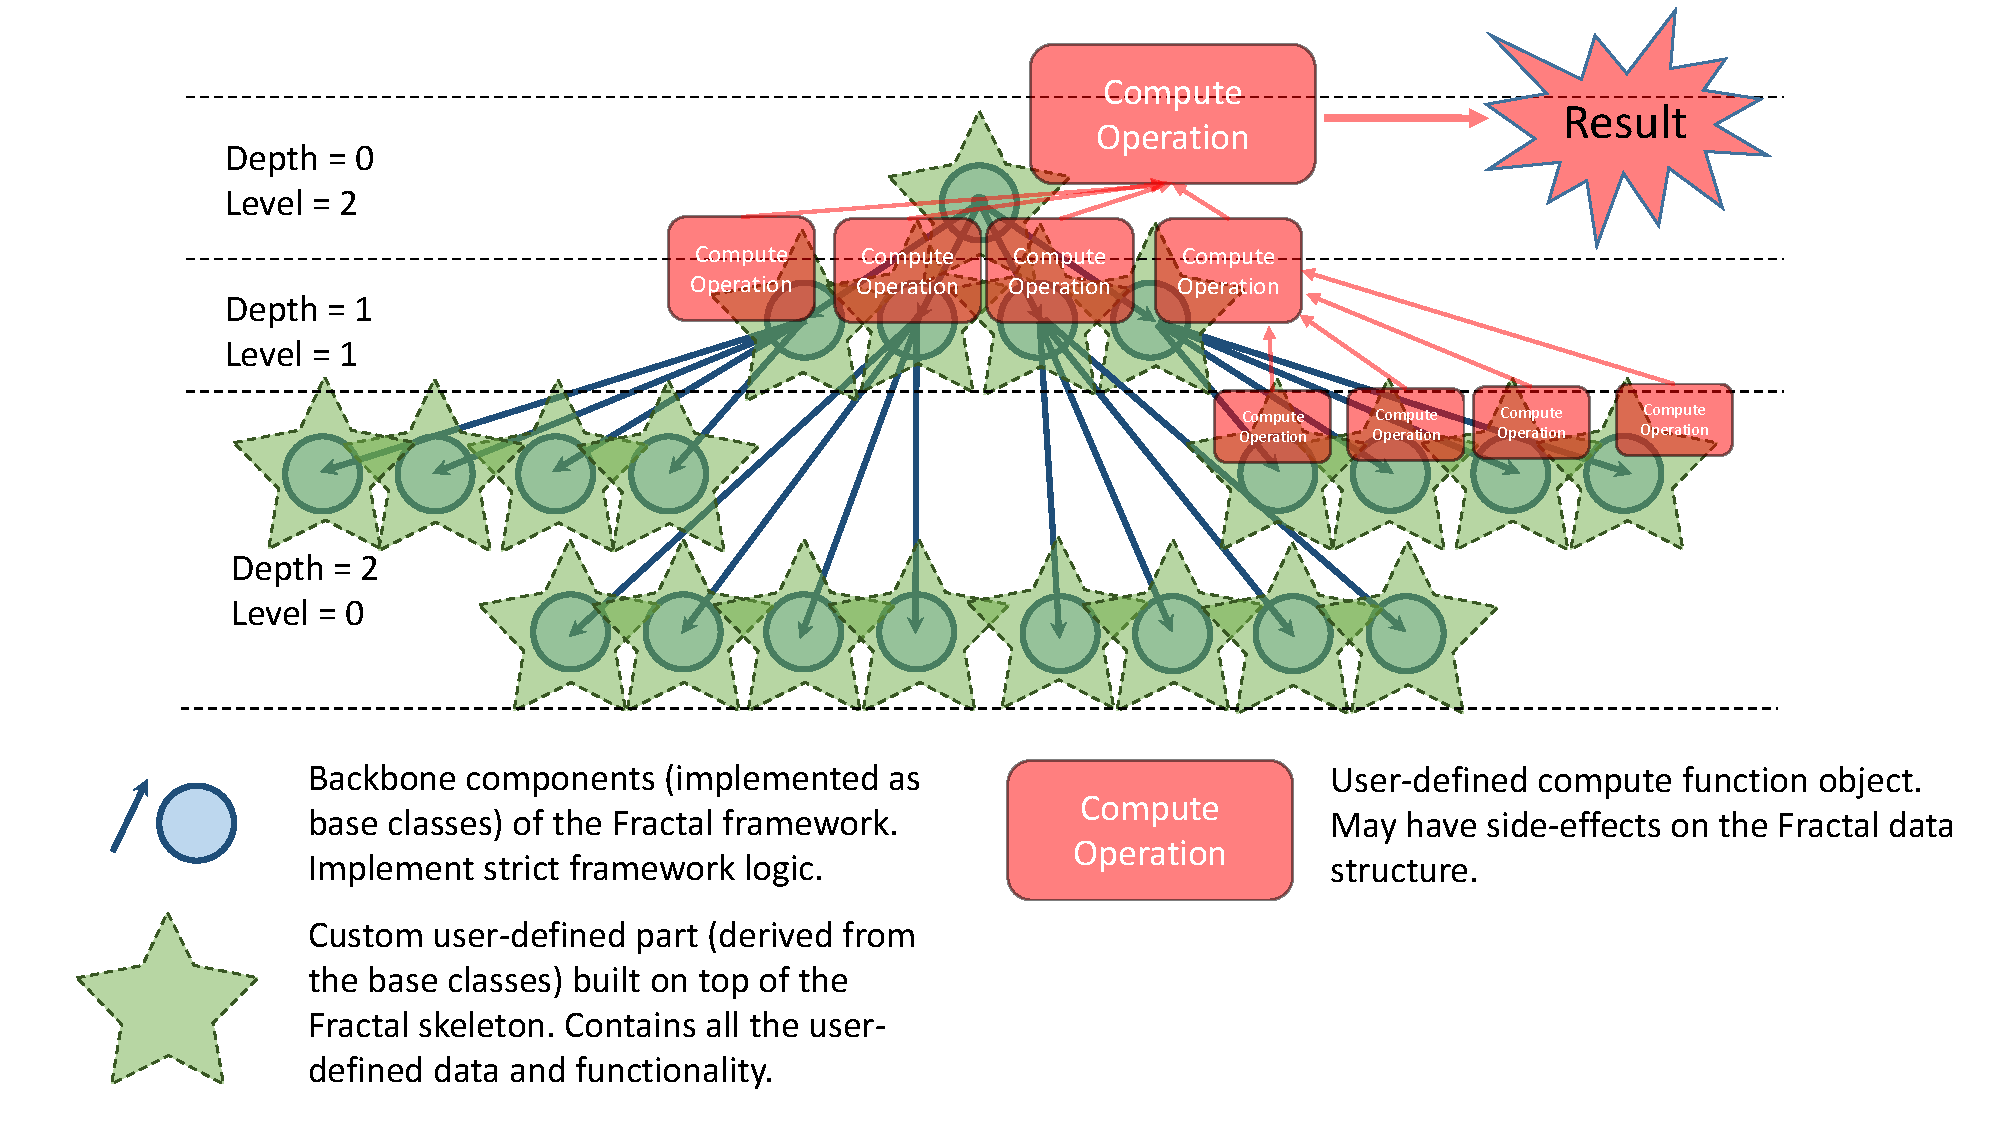
\includegraphics[width=1.0\textwidth]{images/Fractal.pdf}
\caption{The Fractal computational framework.}
\label{fig:fractal}
\end{figure}
\quad A more complicated and interesting fractal example would be a square being continuously and recursively divided into 4 equal sub-squares (southwest, northwest, southeast and northeast). The deep-growing structure is actually a 4-ary tree as well. Imagine one wants to compute the perimeter of some figure. One way to do it would be to map the figure on the square plane and then turn the plane into a grid by continuously splitting the square into 4 equal sub-parts (southwest, northwest, southeast, northeast) till we reach the granularity size of the grid. Then we paint all the grid elements located inside the figure shape as black and those outside of it as white. We iterate over the grid and detect all points of color flips and add the size of the grid elements to the final sum, which at the end is going to approximate the perimeter of the figure. That is roughly what the perimeter benchmark does.\newline\null
\quad In all its generality the fractal is a pattern, which can be characterized with self-similarity, repeatedness, structuredness, inherent parallelizability and the exact numeric values such as its depth and arity. All that naturally maps onto the C++ implementation as a class template we describe below.
\subsection{Fold}
\quad The Fold computational framework has been inspired by the computation done in the power benchmark. The fold is not a new concept and has found a wide application in many functional languages. The C++ language provides std::accumulate() function template as a component of its Standard Template Library, which performs a functional fold over a given data structure, but contrary to our computational framework does not allow any side-effects and modifications to the elements of the data structure. Moreover, our C++ class template library provides an alternative interface to a user with an extensible customization space.\newline\null
\begin{figure}[ht]
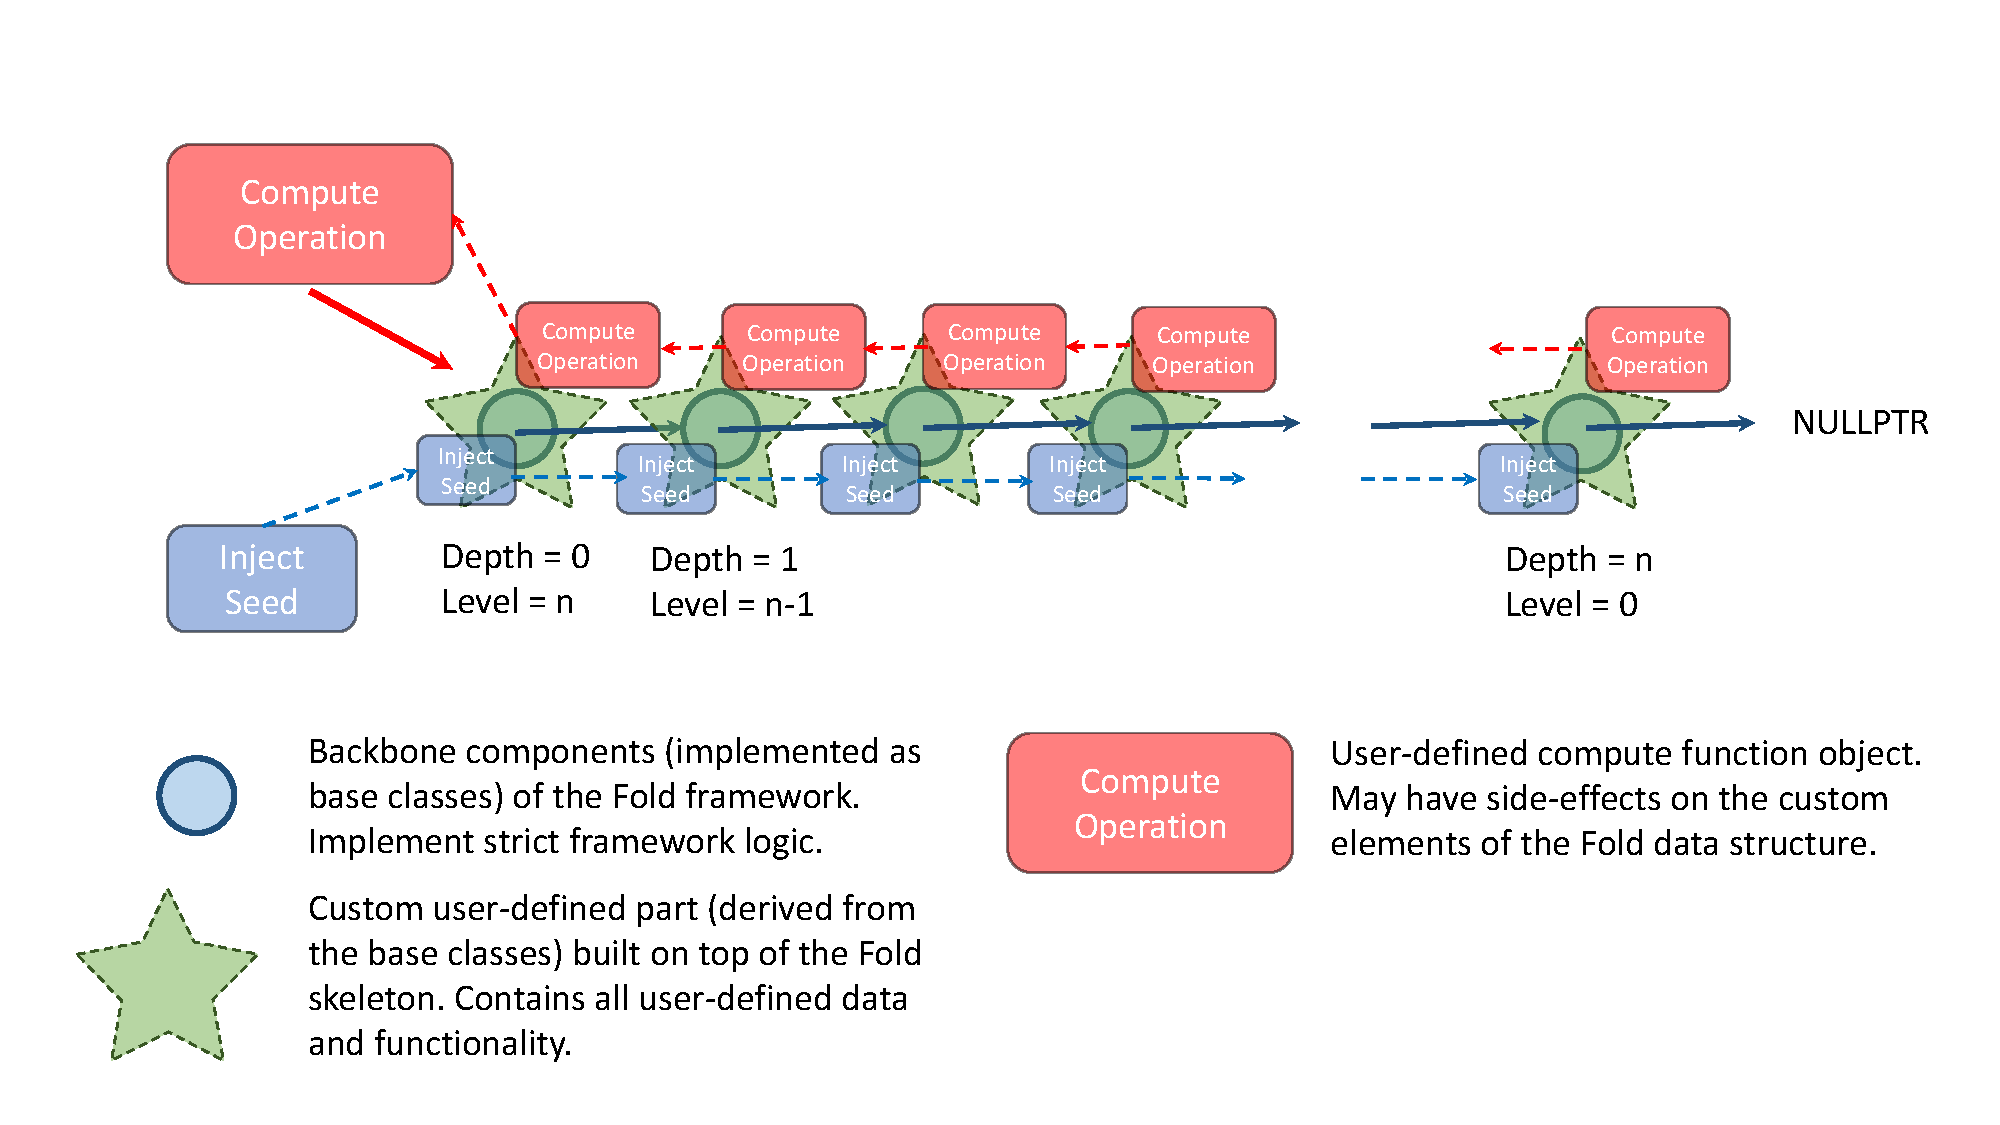
\includegraphics[width=1.0\textwidth]{images/Fold.pdf}
\caption{The Fold computational framework.}
\label{fig:fractal}
\end{figure}
\quad One can think of a Fold as a set of elements arranged into a linked-list. We grow the list to the specified depth given a seed value. Then we may inject some data into the head of the list and propagate it to its tail element. All propagation modifications are user-defined. Once every element of the list is ready with its data, the computation starts at the tail element and passes computed values back to previous elements of the chain.         


\subsection{Reduce}
\quad The Reduce computational framework is a well-known one. The difference between our computational framework and std::reduce() from C++ Standard Template Library (STL) is the possibility of having side effects and an alternative user customization interface. Our computational framework takes a function object with two overloaded and overridden virtual operator() methods. One specifies how to reduce the value from a single element (possibly changing the element in the process) and the other one defines the way of combining all the reduced values into the final return value. Our framework implements sequential as well as parallel Reduce versions.  


\subsection{Frameworks Library Design and Implementation}
\quad The design and implementation of computational frameworks library have been done iteratively using 4 Olden benchmarks as inspiration and  
The design of the C++ computational frameworks library aims at several goals.  
\begin{description}
\item[Modern C++] The implementation of the library is based on the Standard Template Library (STL) data structures, uses move semantics and unique pointers to achieve efficiency and smart memory management. For parallelization library uses OpenMP standard. All that provides for a wide source-code portability. The library is composed of a set of header files with class templates, which are supposed to be included into the user application.  
\item[Convenience] 
\item[Coherence] All computational frameworks in the library share the same user interface as well as internal design. Frameworks are inter-operable and flexible: one can create say, a fold of fractals of reductions. Different components can compute different return types.

\item[Sound design] CRTP, Algorithm Template pattern
\end{description}
\quad The computational frameworks are designed as a set of C++ class templates. The user interface these templates provide has been designed and refined iteratively using the set of Olden benchmarks [].     

\begin{minipage}[t]{\linewidth}
\begin{lstlisting}[caption={Computational framework class template skeleton},label={lst:framework_template_skeleton},language=C++]

template <typename ElemType, typename SeedType>
class Framework {
    public:
        class Element {
            // user-exposed customization iface
            virtual void grow(SeedType) = 0;
            virtual bool growth_stop_condition() { return false; }
        };
        template <typename ComputeType>
        class ComputeFunction {
            // framework specific application function API
            virtual operator()(ElemType& elem, ... ) = 0;
            virtual operator(const std::vector<ComputeType>&) = 0;
*       };
   /     
        void grow(size_t size, SeedType seed) {
            // organise framework elements 
            // into a data structure
            ... = new ElemType(); 
        }
        template<typename ComputeType>
        ComputeType compute(ComputeFunction<ComputeType>& apply_func);
    
    private:
        // framework data structure organisation
        // (list, tree, array, etc.)
};

\end{lstlisting}
\end{minipage}

\quad The design and the implementation of our template library reflect the target goals of the concept of computational frameworks.    

\quad There were several questions raised in the design process of a template library. 

\section{Performance of the library}
\quad We have rewritten old legacy C implementations of 4 Olden benchmarks: health, perimeter, treeadd and power. The table below shows the performance gains our versions have over old sequential implementations.   




